\chapter{Architecture}
\label{chap:architecture}

This chapter will define the architecture of the tool being proposed. It will begin by describing the technology to be utilised in its implementation, so as to narrow down the possible architectural styles and patterns that can be applied in its construction.

%----------------------------------------------

\section{Technology}

In order to properly define Atlas' architecture, it is necessary to first study the technology that is available for its implementation, as this should narrow down the options of architectural styles and patterns that can be applied \cite{TAYLOR:2009}. This section presents the areas of technology that must be studied in order to identify the appropriate tools, languages and other instruments to be used in Atlas' implementation.

%----------------------------------------------

\subsection{Diagramming Libraries}
\label{sec:diaglibs}

The primary function of Atlas is that of permitting the graphical diagramming of Feature Models within a Web-based environment. In order to minimise effort, as well as standing in accordance with the precepts of Component-Based Software Engineering (CBSE) \cite{JIFENG:2005} \cite{CRNKOVIC:2002a}, it is necessary to identify the currently available libraries that may suit this particular function.

In order to facilitate the research into this subject, certain constraints are established upon this requirement, as follows:

\begin{itemize}
    \item The library's output must be HTTP-compatible, so as to be usable within a Web-environment;
    \item The library must be free for use, as per established requirements;
    \item The library must have sufficient source material to permit its use without trial-and-error implementation;
    \item The library should be proven to work on all modern Web Browsers (Mozilla Firefox, Google Chrome, Internet Explorer, Safari).
\end{itemize}

%----------------------------------------------

\subsection{Client-side Programming Language - CSPL}

Atlas will require use of a programming language engineered for Web environments, so as to permit easy parsing of its client-side service with existing Web Browser technologies. The choices of language will be largely limited by the choices of Diagramming Libraries studied, and should be researched in conjunction with them. The choice of client-side programming language is constrained in the same manner as the Diagramming Libraries.

%----------------------------------------------

\subsection{Database Management System - DBMS}

One of the greatest contributions of the Atlas project is the notion of a free repository of feature models, as well as private feature model repositories per account, should this functionality be passed by project management. For this to be possible, a Database Management System must be selected to persist and provide access to the models.

There is only one constraint upon the DBMS choice, and that is that the DBMS permit an equivalent representation to those used in the Server-side Programming Language, preferably object-oriented collections or entity-relationship models.

%----------------------------------------------

\subsection{Server-side Programming Language - SSPL}

The server-side of Atlas will be largely responsible for the serialising and de-serialising of persisted feature models, as well as offering validation of feature models, executing the transformation between notations and controlling access permissions to the repository database. Therefore, the research of this subject should be constrained by certain premises, as follows:

\begin{itemize}
    \item The language should be capable of processing large data structures, as certain feature models may exceed the tens of thousands of elements and will need to be validated in reasonable time;
    \item It should be possible to program data structures in an object-oriented form, or some similar form that permits reuse of data structure elements;
    \item The language must be capable of accessing the DBMS selected for the repository;
    \item The language must be capable of providing a Web server to communicate through HTTP packets with the Client-side service.
\end{itemize}

%----------------------------------------------

\subsection{Web Server}

A Web server will need to be installed and configured to provide the Server-side services of Atlas. This Web server must be capable of handling both the SSPL and DBMS choices, as it is likely that we will not avail of the resources necessary to establish two Web servers, and a single one will most likely have to handle the server-side services and persistence of the system. The Web servers researched must also be capable of running on either a Linux or Windows platform, as these are more widely available and therefore of easier maintenance and evolution.

%----------------------------------------------

\subsection{Integrated Development Environment - IDE}

For the better use of human resources in the project, one or two IDE will have to be selected for use between all development team members. The choice of IDE will evidently be limited by the choice of CSPL and SSPL, but it is not required that a single IDE be used for both server-side and client-side development. Whether it be a single one, or two different ones, the IDE responsible for the client-side development must be capable of handling HTML and CSS markup, so as to centralize the development of the application services of the client-side.

%----------------------------------------------

\section{Architectural Style}

This section will present the architectural styles selected for use in the design of Atlas' architecture.

%----------------------------------------------

\subsection{Client-Server}

Due to the distributed nature of both Atlas and the overarching Hestia project, it is clear that the primary architectural style used should be the Client-Server style. The further study of this style is necessary for the full design of Atlas' architecture.

%----------------------------------------------

\subsection{Blackboard}

At the current time, December 10th, 2016, the authors believe it prudent to assume that a Blackboard-like architectural style be adequate for the implementation of the GUI of the client-side application. Further study of this style, as well as selection of a diagramming technology to be used in the implementation, should clarify whether or not this style is indeed adequate for this application.

%----------------------------------------------

\section{Architecture Views}

This section presents the views of the Atlas architecture, the relations between them and the specifications of their elements. These views are at the time presented primarily in UML diagrams \cite{OMG:2011}, along with certain semantically-loose freehand diagrams.

%----------------------------------------------

\subsection{Overview}

The overview of Atlas serves to present the highest-level concepts of the system's architecture, including the form of software deployment and the high-level interfaces of each high-level component.

\subsubsection{High-level Deployment Diagram}

The basic elements of the Overview can be divided between the Client and Server components, as presented in Figure \ref{fig_overview}. The Client is responsible solely for maintaining its own model of the diagram being modeled by the user, as well as the GUI functions, separated between the presentation itself, a Renderer component and a State-Machine component. The Server is responsible for maintaining a persistent repository of models and validating models provided by the Clients.

\begin{figure}[ht]
    \centering
        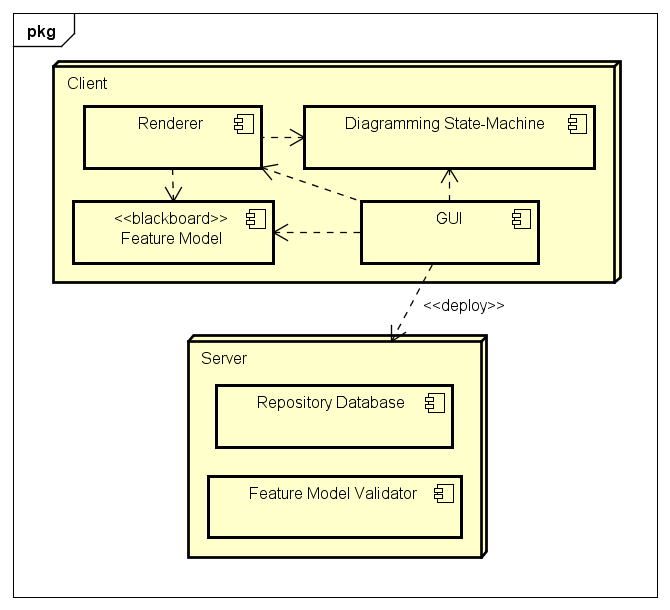
\includegraphics[scale=0.65]{figures/Overview.png}
	\caption{High-level Deployment Diagram}
	\label{fig_overview}
\end{figure}

\subsubsection{High-level Client Component Diagram}

The client can be further defined by establishing the interfaces provided and consumed by its components, as well as by defining the GUI as a subsystem and establishing its inner parts. This is presented in Figure \ref{fig_client}. As can be seen, the GUI subsystem redirects all of its parts' requests to the appropriate interfaces, encapsulating the Model Visualizer, Diagramming Toolbar and System Interface components. Furthermore, both the Renderer and the GUI access the Feature Model through the same \textit{Façade} component; likewise the Diagramming State-Machine. This enables these components (Feature Model; Diagramming State-Machine) to provide services independently of application, expanding their re-usability.

\begin{figure}[ht]
    \centering
        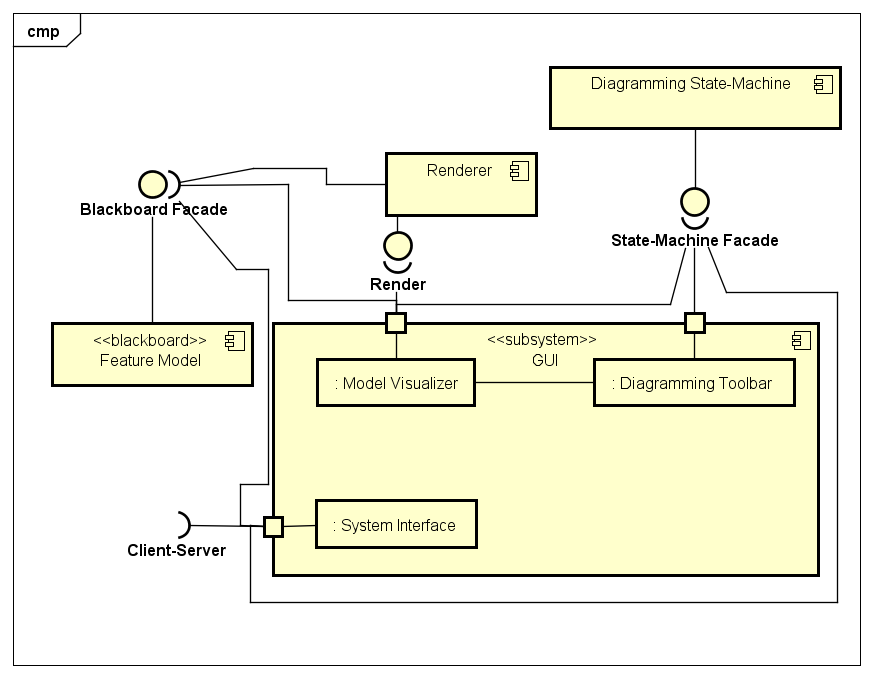
\includegraphics[scale=0.52]{figures/Client.png}
	\caption{High-level Client Component Diagram}
	\label{fig_client}
\end{figure}

\subsubsection{High-level Server Component Diagram}

The server is not as well-defined as the client, presenting a simple Linkage connector that permits the Client to access it through a single entry-point for both of its functions. This is presented in Figure \ref{fig_server}.

\begin{figure}[ht]
    \centering
        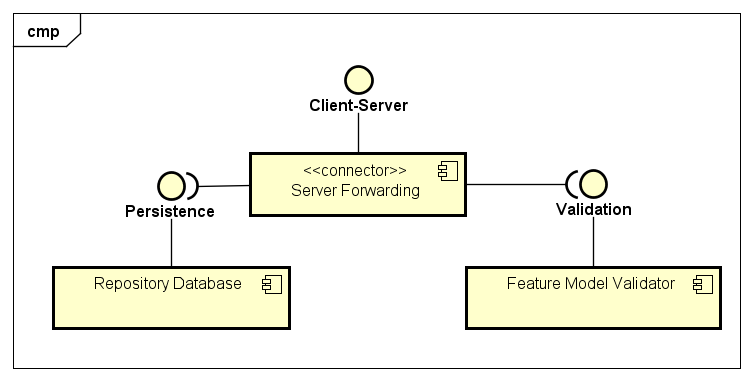
\includegraphics[scale=0.6]{figures/Server.png}
	\caption{High-level Server Component Diagram}
	\label{fig_server}
\end{figure}

%----------------------------------------------

\subsection{State-Machine View}

Due to the complexity of the State-Machine, a comprehensive description of it will be provided in this section, in the form of natural language descriptions and UML Statechart diagrams. Different views are provided for each Feature Model notation, given that the operations available in them can differ greatly.

%----------------------------------------------

\section{Client Component Specifications}

The client side of the Atlas application is formed by four main components: Diagramming State-Machine; Renderer; Feature Model, and; GUI. The GUI subsystem can be further reduced to the sub-components: Model Visualizer; Diagramming Toolbar, and; System Interface. This section presents the specification of each of these components in natural language, as well as a freehand code-like representation of each component's interfaces, loosely based on the OMG IDL \cite{OMG:2014}.

%----------------------------------------------

\subsection{Diagramming State-Machine}

The Diagramming State-Machine component serves to maintain the current state of the diagramming application in accordance to the interactions of the user with the GUI, primarily with the Diagramming Toolbar and Model Visualizer. The states held by this component are then used by the GUI to define which operations are permitted upon the model.

\begin{listing}
\begin{minted}[xleftmargin=21pt,
                breaklines=true,
                tabsize=4]{text} 
State-Machine Facade{
    property state cState;
    property operation[] aOperations;

    out state currentState(){ 
        return cState; 
        };
    inout state transition(operation t){
        execute t;
        return cState;
        };
    out operation[] availableOperations(){
        return aOperations;
        };
    out boolean isAvailable(operation t){
        return true if (t exists in aOperations)
                    else false;
        };
}
\end{minted}
\caption{Representation of State-Machine Facade}
\label{list:smFacade}
\end{listing}

This component provides a single \textit{Façade} type interface offering: a \textit{get} operation for the current state; a \textit{transition} operation for modifying the state, and; permission operations that inform which operations are available from a certain state, or whether or not a certain operation is available. Listing \ref{list:smFacade} presents a code-like representation of this interface.

%----------------------------------------------

\subsection{Renderer}

The Renderer component serves as an encapsulation of the diagramming library functions used to render the visualization of the model. It operates based on a procedure call connector linked to the GUI, which activates the Renderer, and the \textit{Façade} type interface provided by the Feature Model blackboard. This component holds no internal state, being responsible solely for providing operations and accessing the blackboard model. Listing \ref{list:render} presents a code-like representation of the Render interface.

\begin{listing}
\begin{minted}[xleftmargin=21pt,
                breaklines=true,
                tabsize=4]{text} 
Render{
    out visualization render(){
        execute create visualization v;
        return v;
    }
}
\end{minted}
\caption{Representation of Render interface}
\label{list:render}
\end{listing}

The interaction of the Render component with the Feature Model blackboard is read-only, being responsible solely for creating a visualization from the model.

%----------------------------------------------

\subsection{Feature Model}

The Feature Model component serves as a blackboard model to the client application. It holds the entire structure of the model being constructed, as well as any data required for visualization rendering. It is modified in accordance to the user's interaction with the GUI, in accordance to permissions given by the Diagramming State-Machine, and serves as the basis for the actions of the Renderer.

\begin{listing}
\begin{minted}[xleftmargin=21pt,
                breaklines=true,
                tabsize=4]{text} 
Feature Model Facade{
    property model;

    in void alter(operation t, elements[] e){
        execute operation t(e);
    }
    out model view(){
        return model;
    }
}
\end{minted}
\caption{Representation of Blackboard Facade}
\label{list:fmFacade}
\end{listing}

Listing \ref{list:fmFacade} presents a code-like representation of the Blackboard Facade interface. It is important to note that this representation is highly abstract, assuming that all operations have a single related procedure with a well-specified signature. In practice, operation overloading is probable and proper care must be taken during implementation. It is also important to note that only the GUI has access to the \textit{alter} operation, this being forbidden to the Renderer.

%----------------------------------------------

\subsection{GUI}

The GUI is a subsystem within the client application of Atlas, serving as an encapsulation for the inner GUI components. Given that no interfaces are provided by the GUI subsystem, the external components need not know whence requests originate from, interaction with the GUI subsystem which forwards the responses appropriately, based on the port/interface used for the request. The GUI subsystem is responsible for the visualization of the Feature Model, as well as handling the user interactions in what refers to both diagramming actions and system actions, as defined below.

%----------------------------------------------

\subsubsection{Model Visualizer}

The Model Visualizer sub-component is strictly responsible for presenting the visualization of the Feature Model, as provided by the Renderer, executing tooltip and highlight type operations based on the current state of the State-Machine and cursor position, and acquiring cursor coordinates. The Model Visualizer is therefore not responsible for holding the model being presented, and is encapsulated away from GUI buttons that interact with the State-Machine and the server.

This component's interactions can be divided between the interfaces it consumes:

\begin{itemize}
    \item The State-Machine is used by the Model Visualizer to identify the which state is currently active, and to execute operations that require cursor coordinate input. The information of active state is used to decide what tooltip and highlight operations must be executed depending on cursor position. The operations executed upon the State-Machine from the Model Visualizer will not forward the cursor coordinates, but rather will use them to modify the model in accordance to the state resulting from the operation. Unlike the Diagramming Toolbar, the Model Visualizer is NOT responsible for identifying whether or not an operation is legal prior to forwarding it to the State-Machine. Rather, it must be capable of treating exceptions, undoing recent operations, and presenting help messages to the user.
    
    \item The Renderer is used by the Model Visualizer when, upon executing an action, it identifies that the current state of the State-Machine requires a re-drawing of the visualization.
    
    \item The Blackboard is used by the Model Visualizer when, upon executing an action, it identifies that the current state of the State-Machine requires updating the model.
\end{itemize}

%----------------------------------------------

\subsubsection{Diagramming Toolbar}

The Diagramming Toolbar sub-component serves strictly to encapsulate operations executed upon the State-Machine which do not require cursor coordinate input. Generally speaking, it will operate sequentially, forwarding a (previously-identified as legal) operation to the State-Machine, and then reforming the presented Toolbar in accordance to what operations are legal after the operation is executed. The Diagramming Toolbar is responsible for identifying whether or not an operation is legal prior to forwarding it to the State-Machine.

%----------------------------------------------

\subsubsection{System Interface}

The System Interface sub-component is responsible for all communication between client and server. Therefore, all operations that depend upon the persistence repository or the model validators must be represented in the System Interface GUI. Despite being part of the GUI, the System Interface sub-component is independent from the Model Visualizer and Diagramming Toolbar sub-components, operating strictly based on the Blackboard state and the operations provided by the server. The exception are the initialization operations (Load Model, New Model), which force change the State-Machine and force starts the Renderer.